\documentclass{article}

\usepackage{ctex}
\usepackage{tikz}
\usetikzlibrary{cd}

\usepackage{amsthm}
\usepackage{amsmath}
\usepackage{amssymb}

%\usepackage{unicode-math}


\usepackage[textwidth=18cm]{geometry} % 设置页宽=18

\usepackage{blindtext}
\usepackage{bm}
\parindent=0pt
\setlength{\parindent}{2em} 
\usepackage{indentfirst}

\usepackage{listings}
%\usepackage{minted}% hightlighting

\usepackage{proof} % infer

\usepackage{xcolor}
\usepackage{titlesec}
\titleformat{\section}[block]{\color{blue}\Large\bfseries\filcenter}{}{1em}{}
\titleformat{\subsection}[hang]{\color{red}\Large\bfseries}{}{0em}{}
%\setcounter{secnumdepth}{1} %section 序号

\newtheorem{theorem}{Theorem}[section]
\newtheorem{lemma}[theorem]{Lemma}
\newtheorem{corollary}[theorem]{Corollary}
\newtheorem{proposition}[theorem]{Proposition}
\newtheorem{example}[theorem]{Example}
\newtheorem{definition}[theorem]{Definition}
\newtheorem{remark}[theorem]{Remark}
\newtheorem{exercise}{Exercise}[section]
\newtheorem{annotation}[theorem]{Annotation}

\newcommand*{\xfunc}[4]{{#2}\colon{#3}{#1}{#4}}
\newcommand*{\func}[3]{\xfunc{\to}{#1}{#2}{#3}}

\newcommand\Set[2]{\{\,#1\mid#2\,\}} %集合
\newcommand\SET[2]{\Set{#1}{\text{#2}}} %

\begin{document}
\title{Abstract Interpretation}
\author{枫聆}
\maketitle
\tableofcontents

\section{Motivation}

单调分析框架的诞生让做程序分析的人可以构造一个精准的,数学形式化的分析. 在这个框架下,我们需要一个lattice domain,每个instruction相关联的transfer functuons和一个初始的状态. 几乎先有的程序分析手法都可以总结到这个单调分析框架上.

那么抽象解释可以理解为在单调分析框架上又迈出了一步. 我们经常的设计分析思路:开始从一个简单的分析开始,分析结果的正确性可以很容易得到证明. 这里的分析是指collecting semantics,即从程序的语义里面收集我们想要的信息. 最开始的分析一般来说,我们的想法是非常的理想导致它的可行性或者可计算性是比较难处理的或者说根本不可能处理,因为有可能我们关注的property所在lattice对应的underlying set的基数是比较大的,或者不满足一些良好的性质例如ACC. 因此我们尝试使用近似计算的方法,把property所在的lattice变小,这个过程可能是一个迭代的过程,直到我们最终可以计算为止或者达到一个理想的效果. 而抽象解释就是提供这样一种系统的方法来帮助我们.

%实际分析domain太复杂,也许这个实际分析domain满足一些不错的性质比如ACC等等,但是还是掩盖不了它过于复杂. 所以我们尝试使用某个抽象的domain来代替分析,这个抽象的domain要比实际分析的domain更小,我们分析起来更加得心应手,但是问题是如何构造这个抽象的domain? 它分析出来的结果是否可以作为真的truth? 它的结果能在多大程度上说明一些问题? 后期我们是否可以考虑优化抽象的domain来让结果更好一点?


\newpage
\section{Correctness Relations}

\begin{definition}
\rm {\color{red} (Correctness relations).} A relation $R \subseteq V \times L$ is said to be a correctness relation iff it satifies the following two conditions:
\begin{enumerate}
	\item $\forall v \in V,l_1,l_2 \in L,~(v~\mathcal{R}~l_1)~\text{and}~(l_1 \leq l_2) \rightarrow (v~\mathcal{R}~l_2);$
	\item $\forall v, \forall L' \subseteq L,~(\forall l \in L',~(v~ \mathcal{R}~l)) \rightarrow v~\mathcal{R}~(\bigwedge L').$
\end{enumerate} 

{\color{red} 这里$V$表示concrete values,$L$表示abstract values构成的lattice. $v~\mathcal{R}~l_1$表示$l_1$是$v$的一个approximation}.

{\color{blue} 用自然语言来描述就是(1) 若$v$对应某个$l_1$,那么对于$l_1$的一个upper approximation $l_2$, 有$v \in l_2$. (2) 若$v$同时对应多个abstract values,这里应该是一个and的关系,那么$v$可以对应它们的一个greatest lower bound}.
\end{definition}


\begin{lemma}
\rm If $\mathcal{R} \subseteq V \times L$ is a correctness relation, then
$$
\begin{aligned}
& v~\mathcal{R}~\top \\
& (v~\mathcal{R}~l_1)~\text{and}~(v~\mathcal{R}~l_2) \rightarrow v~\mathcal{R}~(l_1 \wedge l_2) \\
& (v~\mathcal{R}~l_1)~\text{or}~(v~\mathcal{R}~l_2) \rightarrow v~\mathcal{R}~(l_1 \vee l_2)
\end{aligned}
$$
\end{lemma}

前面简单的描述了一下correctness relation操作含义,但是correctness relation中依然模糊是它里面的lattice到底在刻画一个怎样东西? 我们的分析中为什么要引入lattice? 为了让这个lattice is reasonable,我们来具体定义这个lattice的meet和join操作的内在含义.

\begin{definition}
\rm we need the meet and the join operator in order to combine abstract values: 
\begin{enumerate}
	\item If a value is described by both $l_1$ and $l_2$, by combine these two properties, we obtain the more precise information $l_1 \wedge l_2$.
	\item If a value is described by either $l_1$ or $l_2$, the most precise info that we can infer is $l_1 \vee l_2$. 
\end{enumerate}

{\color{blue}在上面定义的operations的内在含义下,smaller代表更精准,bigger代表更安全,更安全就是指考虑的更全面,不会丢掉信息而造成一些潜在的问题. $\wedge$等价于逻辑连词的and,$\vee$等价于逻辑连词的or. 在实际分析的过程中$\wedge$和$\vee$这两个operations就要针对我们关注的properties来具体定义,但是它的最本质内在含义是每次都是尽可能在不丢失精确度的可能下,去尽可能的提高结果本身的精确度}.
\end{definition}


\newpage
\begin{annotation}
\rm {\color{red} 如何取证明一个分析的正确性} To prove the correctness of the analysis, it is su±cient to prove 
\begin{enumerate}
	\item The initial property (abstract state) $l_0$ is a correct approximation of the initial value (concrete state) $v_0: v_0~\mathcal{R}~ l_0$.
	\item Each transition preserves the correctness relation
	$$
	\forall v_1,v_2,l_1,l_2,~(v_1 \rightsquigarrow v_2)~\text{and}~(v_1 ~\mathcal{R}~l_1)~\text{and}~(f_L(l_1) = l_2) \rightarrow v_2~\mathcal{R}~ l_2.
	$$
\end{enumerate}
{\color{blue} 用自然语言来描述就是你首先要保证初始状态下correctness relation的存在,而后在状态传递的过程中这个correctness relation 依然是保持的,这个过程就关系到两个传递函数concrete value transfer function和abstract value transfer function}.
\end{annotation}


\newpage
\section{Galois connections}

\begin{annotation}
\rm 数学家们经常在思考面临一个场景: 有两个“世界”和两个转换函数作为这个两个世界的连接。 更甚之,如果其中某个世界中的对象经过转换到另外一个世界中,然后再把这个对象再转换回去,如此往复迭代最终结果是稳定的. 特别地,无论从哪个世界开始,第三次转换的结果和第一次转换的结果是相同的. 

如果这两个世界各自的对象之间着某种自然规律,转换函数在传递过程中遵守这些自然规律. 在类似我们经常碰见的简单或者复杂的场景中,有一种优雅的方式可以尝试来面对它们--Galois connection。
\end{annotation}

关于galois connection我们通常可以看到两个定义,下面我来说明两个定义是等价,也就是说可以从任意一个推出另外一个.

\begin{definition}
\rm {\color{red} nlab上的定义更贴近adjunction的味道} Given posets $A$ and $B$, a Galois connection between $A$ and $B$ is a pair of order-preversing functions $\func{f}{A}{B}$ and $\func{g}{B}{A}$ such that $a \leq g(f(a))$ and $b \geq f(g(b))$ for all $a \in A$, $b \in B$. 

{\color{blue} 注意这里的order-preversing,最原始的定义用的是order-reversing,导致我在这里弄出了一些矛盾}.
\end{definition}

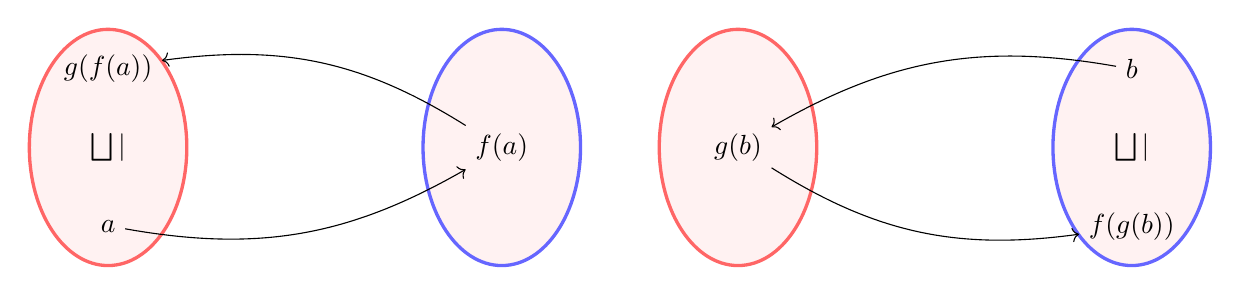
\begin{tikzpicture}
\filldraw[color=red!60, fill=red!5, very thick](-1,0) ellipse (1 and 1.5);
\filldraw[color=blue!60, fill=red!5, very thick](4,0) ellipse (1 and 1.5);
\node (a) at (-1,-1) {$a$};
\node (fa) at (4,0) {$f(a)$};
\node (gfa) at (-1, 1) {$g(f(a))$};
\node (l) at (-1,0) {$\bigsqcup|$};
\draw [->] (a) edge[bend right=20] (fa) (fa) edge[bend right=20] (gfa);

\filldraw[color=red!60, fill=red!5, very thick](7,0) ellipse (1 and 1.5);
\filldraw[color=blue!60, fill=red!5, very thick](12,0) ellipse (1 and 1.5);
\node (b) at (12, 1) {$b$};
\node (gb) at (7,0) {$g(b)$};
\node (fgb) at (12,-1) {$f(g(b))$};
\node (l) at (12,0) {$\bigsqcup|$};
\draw [->] (b) edge[bend right=20] (gb) (gb) edge[bend right=20] (fgb);
\end{tikzpicture}

\begin{proposition}
\rm Given posets $A$ and $B$, a pair of order-preversing functions $\func{f}{A}{B}$ and $\func{g}{B}{A}$ is a Galois connection between $A$ and $B$ if and only if, for all $a \in A$, $b \in B$, we have 
$$
f(a) \leq b~\text{if and only if}~a \leq g(b).
$$
\end{proposition}

\begin{center}
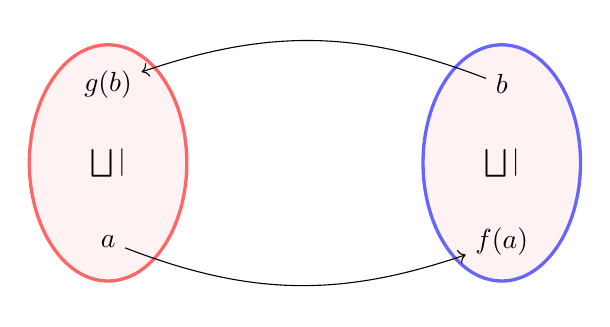
\begin{tikzpicture}
\filldraw[color=red!60, fill=red!5, very thick](-1,0) ellipse (1 and 1.5);
\filldraw[color=blue!60, fill=red!5, very thick](4,0) ellipse (1 and 1.5);
\node (a) at (-1,-1) {$a$};
\node (fa) at (4,-1) {$f(a)$};
\node (b) at (4, 1) {$b$};
\node (gb) at (-1,1) {$g(b)$};
\node (l1) at (-1,0) {$\bigsqcup|$};
\node (l2) at (4,0) {$\bigsqcup|$};
\draw [->] (a) edge[bend right=20] (fa) (b) edge[bend right=20] (gb);
\end{tikzpicture}
\end{center}

\begin{proof}
($\Rightarrow$). 前提$(f,g)$是一个galois connection,给定$a \in A$, $b \in B$. 若$f(a) \leq b$, 两边同时apply $g$, 有$g(f(a)) \leq g(b)$,同时有$a \leq g(f(a))$. 那么$a \leq g(b)$. 若$a \leq g(b)$,同理可以得到$f(a) \leq b$.

($\Leftarrow$). 前提$(f,g)$满足$f(a) \leq b~\text{if and only if}~a \leq g(b)$. 我们直接取$b = f(a)$, 那么$f(a) \leq f(b)$当且仅当$a \leq g(f(a))$. 同理直接取$a = g(b)$,那么$g(b) \leq g(b)$当且仅当$f(g(a)) \leq b $.   
\end{proof}

{\color{blue} 关于adjunction的东西$fg \rightarrow id$和$gf \rightarrow id$,这个箭头是一个natural transform, 至于更细的东西要去看看category theory了! PAAA上说$f$和$g$互为“weak inverse”,看起来也是比较形象啊!所以有下面的一个命题}.

\begin{annotation}
\rm 现在我们尝试把galois connection放到抽象解释范畴上,让lattice $A$表示我们原本一个analysis domain,lattice $B$表示一个更抽象的analysis domain用来加快我们的分析或者让我们的分析可计算,那么这里$\func{f}{A}{B}$称为{\color{red} abstraction function},$\func{g}{B}{A}$称为{\color{red} concretization function}. 

这里的$f$和$g$都是单调函数意味,原本的实际值之间的关系在abstract domain上依然保持,反过来亦然,同时galois connection强化的两个条件
\begin{enumerate}
	\item $a \leq g(f(a))$表示抽象过程是可能会丢失精度的,但是依然是正确的. {\color{blue} 我的理解是把具体的值通过映射放到抽象域里面做运算得到的结果,再映射回来可能比在具体域里面做运算得到的结果要稍微差一点,但是正确性是可以保证的}.
	\item $b \geq f(g(b)$表示具体化的过程不会丢失精度. {\color{blue} 本来抽象值,放到具体域里面操作一遍,再映回来是不会丢精度,这也是可以很自然想到的}.
\end{enumerate}
如果更细致去刻画一下我自己的annotation就是
\begin{enumerate}
	\item $x,y \in A$
	$$
	x \vee y \leq g(f(x) \vee f(y)).
	$$
	\item $x',y'\in B$
	$$
	x' \wedge y' \geq f(g(x) \wedge g(y)).
	$$
\end{enumerate}
为此我们需要去分别证明$f(x \vee y) = f(x) \vee f(y)$和$g(x \wedge y) = g(x) \wedge g(y)$.
\end{annotation}



\newpage

\begin{proposition}
\rm {\color{red} (Galois connection引发的semilattice homomorphism)} For a Galois connection $(f,g)$ of lattice $A$ and $B$, $f$ preserves finite join:
\begin{enumerate}
	\item $f(\perp_A) = \perp_B$;
	\item $f(x \vee y) = f(x) \vee f(y)$.
\end{enumerate}
And similarly 
\begin{enumerate}
	\item $g(\top_B) = \top_A$;
	\item $g(x \wedge y) = g(x) \wedge g(y)$.
\end{enumerate}

{\color{blue} 啧啧,没想到啊galois connection竟然弄了一个semilattice homomorphism出来,突然想找一下characterization of semilattice homomorphism}. 
\end{proposition}

\begin{proof}
(1) 由于$B$上$\perp_B$的性质,有$f(\perp_A) \geq \perp_B$. 反过来由于$A$上的$\perp_A$性质,有$g(\perp_B) \geq \perp_A$,再用一下galois connection的性质,有$f(\perp_A) \leq \perp_B$. 综上两边夹,所以$f(\perp_A) = \perp_B$.

(2) 由于$f$是monotone,有$f(x) \leq f(x \vee y)$和$f(x) \leq f(x \vee y)$,所以$f(x) \vee f(y) \leq f(x \vee y)$是一个upper bound. 最关键是确界证明$f(x \vee y) \leq f(x) \vee f(y)$. 由于galois connection,有$x \leq g(f(x))$,再由$g$是monotone,有$x \leq g(f(x) \vee f(y))$. 同理也有$y \leq g(f(x') \vee f(y'))$,那么
$$
x \vee y \leq g(f(x) \vee f(y))
$$
再用一下galois connection,就有$f(x \vee y) \leq f(x) \vee f(y)$. 综上两边夹,所以$f(x \vee y) = f(x) \vee f(y)$. {\color{red} 值得关注是$f$和$g$都只是一个semilattice homomorphism,而且是两种不同操作}. 其实我们做分析的时候,也只是使用一个semilattice,至于是meet还是join和原本分析过程的方向是有关的. 
\end{proof}

\begin{proposition}
\rm {\color{red} (weak inverse)} For galois connection $(f,g)$, we have the equations
$$
\begin{aligned}
f \circ g \circ f  = f \\
g \circ f \circ g = g.
\end{aligned}
$$

{\color{blue} 这个命题内在是在说明你把分析结果用$f$和$g$进行迭代是不会改变精度的!}
\end{proposition}

\begin{proof}
(1).
$$
\begin{array}{cc}
 f(a) \leq  f \circ (g \circ f(a)) & {\color{red} f \circ( g \circ f)} \\
 (f\circ g) \circ f(a) \leq f(a) & {\color{red}(f \circ g) \circ f}, \\
\end{array}
$$
所以$f \circ g \circ f  = f$. 同理可证第二个式子.
\end{proof}

\begin{proposition}
\rm {\color{red} ($f$和$g$相互确定)} If the pair $(f,g)$ is Galois connection of join semlattice $A$ and $B$. Then $f$ uniquely determines $g$ by
$$
g(b) = \bigvee\Set{a}{f(a) \leq b}.
$$
and $g$ uniquely determines $f$ by
$$
f(a) = \bigwedge\Set{b}{a \leq g(b)}.
$$

{\color{blue} 我个人认为这个性质真的非常好}!
\end{proposition}


\begin{proof}
对于$g(b)$有
$$
g(b) = \bigvee\Set{a}{a \leq g(b)} = \bigvee\Set{a}{f(a) \leq b}.
$$
那么还要取证明$g$是唯一的,即若存在$g_1$,那么对于任意的$b \in B$,应该有$g(b) = g_1(b)$. 因为
$$
g(b) \leq (g_1\circ f)\circ g(b) = g_1 \circ (f \circ g)(b) \leq g_1(b). 
$$
再把$g$和$g_1$反过来用一遍也可以得到$g_1(b) \leq g(b)$. 所以有$g(b) = g_1(b)$.
\end{proof}

\begin{lemma}
\rm {\color{red} (Galois connection的一种构造方式)} If $\func{f}{A}{B}$ is semilattice homomorphism then there exists $\func{g}{B}{A}$ such that $(f,g)$ is a Galois connection of posets ({\color{red} complete semilattice}) $A$ and $B$.
\end{lemma}

\begin{proof}
假设$f$是一个join semilattice homomorphism. 那么$f$也是monotone的,我们得用$f$来定义$g$
$$
g(b) = \bigvee\Set{a}{f(a) \leq b}
$$
显然$g$是一个单调函数,最重要的是
$$
g(f(a)) = \bigvee\Set{a'}{f(a') \leq f(a)} \geq a .
$$
因为显然$a \in \Set{a'}{f(a') \leq f(a)}$. 我们再反过来考虑
$$
f(g(b)) = f(\bigvee\Set{a}{f(a) \leq b}) = \left\{f(a_1)\vee \cdots \vee f(a_i)\right\}_{a_i \in \Set{a}{f(a) \leq b}} \leq b.
$$
因为$f(a_i) \leq b$.
\end{proof}

\newpage
\subsection{New Analysis: Correctness Relation and Transfer Function}

{\color{red} 这章讲如何把analysis function通过galois connection在analysis domains之间传递}.

\begin{definition}
\rm {\color{red}(新的correctness relations)} The correctness relation $\mathcal{S} \subseteq V \times B$ for the new analysis under Galois connection $(f,g)$ of posets $A$ and $B$ is defined as follows
$$
v~\mathcal{S}~b \iff v~\mathcal{R}~g(b).
$$

{\color{red} 其中的$M$表示新的analysis domain或者说是abstract domain,它还是一个lattice}. {\color{blue} 这里是在说abstract domain上一个correctness relations 当且仅当$g$的作用下是concrete domain上一个correctness relation}.
\end{definition}


\begin{definition}
\rm {\color{red} (新的传递函数)} For the new analysis transfer function, we can choose any function $\func{t_B}{B}{B}$ such that
$$
t_B \geq f \circ t_A \circ g.
$$
where $\func{t_A}{A}{A}$ is analysis function under $A$.
\begin{center}
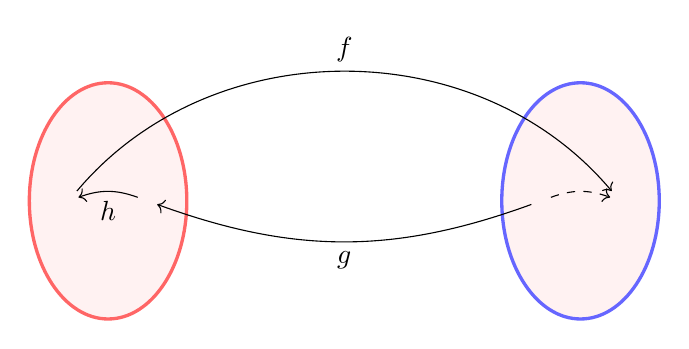
\begin{tikzpicture}
\filldraw[color=red!60, fill=red!5, very thick](-3,0) ellipse (1 and 1.5);
\filldraw[color=blue!60, fill=red!5, very thick](3,0) ellipse (1 and 1.5);

\node (d) at (2.5,0) {} ;
\node (gd) at (-2.5,0) {} ;
\node (hgd) at (-3.5,0) {} ;
\node (fhgd) at (3.5,0) {} ;

\draw [->] (d) edge[bend left=20] node[below] {$g$} (gd) (gd) edge[bend right=20] node[below] {$h$} (hgd); 
\draw [->] (hgd) edge[bend left=50] node[above] {$f$} (fhgd) (d) edge[bend left=20,dashed] (fhgd); 
\end{tikzpicture}
\end{center}
{\color{blue} 但是在实际中我们不会直接通过上面诱导出来的analysis transfer functions $f \circ t_A \circ g$,因为构造起来太过于繁琐,常常会用一个$t_B$来安全的替换它的使用}
\end{definition}



{\color{red} 定义了新的correctness relations和新的analysis tranfer function,我们现在需要来证明这个correctness relations它确实是一个correctness relation,并且$h'$下保持这个relation}.

\begin{proposition}
\rm $\mathcal{S}$ is a correctness relation.
\end{proposition}

\begin{proof}
给定$v \in V$和$b_1,b_2 \in B$且有$b_1 \leq b_2$. 由于$g$是单调的,那么有$g(b_1) \leq g(b_2)$. 若$v~\mathcal{R}~g(b_1) \in A$,那么也有$v~\mathcal{R}~g(b_2)$,即$v~\mathcal{S}~m_2$.

那么再考虑$B' \subseteq B$,若对任意的$b \in B'$都有$v~\mathcal{R}~g(b)$,那么有$v ~\mathcal{R}~(\bigwedge g(b))$,$g$的meet semilattice homomorphism的性质在这里有$v~\mathcal{R}~g(\bigwedge b)$,即$v~\mathcal{S}~(\bigwedge b)$.
\end{proof}

\begin{lemma} \rm {\color{red}(新传递函数是safe的)}
$$
g(t_B(a)) \geq t_A(g(a)).
$$
\end{lemma}

\begin{proof}
$$
g(t_B(a)) \geq (g \circ f)\circ (t_A(g(a))) \geq t_A(g(a)).
$$
\end{proof}

\begin{proposition}
\rm {\color{red}(correctness relations在新传递函数作用下保持)}
$$
\forall v_1,v_2,b_1,b_2,~(v_1 \rightsquigarrow v_2)~\text{and}~(v_1 ~\mathcal{S}~b_1)~\text{and}~(t_B(b_1) = b_2) \rightarrow v_2~\mathcal{S}~ b_2.
$$
\end{proposition}

\begin{proof}
由上面的lemma有
$$
g(b_2) \geq t_A(g(b_1))
$$
所以$v_2~\mathcal{R}~g(b_2)$,即$v_2~\mathcal{R}~b_2$.
\end{proof}

\begin{annotation}
\rm 可以看到Galois connection确实很多的优美的性质,但是想一想实际中我们可能做到这样吗? 是否有必要一定对新的analysis domain构造一个Galois connection?

想象两个analysis domain,都可以很好符合lattice代数结构,并且这两个lattice $A,B$ 还要是complete,通常我们也只考虑finite lattice. Galois connection的存在系统地在$t_A$的基础上诱导出了新的tranfer analysis function $t_B$,而且证明了新构造的correctness relation是正确的,这就是Galois connection起到的重要作用. 我们来具体分析一下在证明它们的过程中哪些是Galois connection导致的直接原因. 

在证明新的correctness relation的时候,第一个条件不需要那么强的条件,只需要$g$单调就行,而第二个条件需要$g$的meet semilattice homomorphism. 而在证明新的tranfer analysis function保持correctness relations过程中需要用到$g \circ f \geq~\text{id}_A$,这个条件也算比较强. 在仔细去分析这些条件的时候,我们就可以感受到我们最确切是需要什么. 那么我们反过来问Galois connection在这里是不是太强了一些?

Salcianu在论文里面提到可以尝试去掉correctness relations的第二个条件,把第二个条件去掉之后我们就不需要$g$保持semilattice homomorphism这么强的条件,为什么可以这样做呢?我们考虑新的abstract analysis domain,实际上它里面的元素和原来的domain是联系比较紧密,并且它们之间是可以天然保持我们感兴趣的关系的,例如把$\mathbb{Z}$换成区间,区间和区间之间定义的包含关系,在对应的lattice上,值和区间关系天然是可以满足更大的 the approximation of 区间继续保持这个关系的. 那么现在来回答Galois connection是不是太强了这个问题,我答案确实是太强了,如果站在我们要去证明一个分析的正确性这个命题而言,它是一个充分条件,而不是必要条件.

前面关于Galois connection构造性命题中,我们在已知一个semilattice homomorphism的情况下,就可以去构造另外一个方向的映射,站在分析的角度而言,我们确实经常有一个semilattice homomorphism介于从concrete domain到abstract domain,但是通常是没有必要把从abstract domain到concrete domain符合Galois connection的映射给构造出来,这也就是上面我们提到的,$g$不需要保持semilattice homomorphism的性质. 但是为了证明新分析过程的正确性我们还是需要$g$是monotone并且$g\circ f \geq ~ \text{id}_A$.
\end{annotation}

%\begin{definition}
%\rm {\color{red} (单调分析框架的定义)} A specification of an analysis in the extended monotone framework is given by
%\begin{itemize}
%	\item an analysis domain $D$ that is semilattice with ordering $\leq$.
%	\item monotone analysis transfer functions $\func{h_n}{D}{D}$ where $n$ is node of program graph.
%	\item an initial element $d_0 \in D$;
%\end{itemize}
%\end{definition}
%
%\begin{definition}
%\rm {\color{red} (Galois connection 诱导出来的analysis function)} A specification of an analysis in the extended monotone framework and a Galois connection $(f,g)$ from $D$ to the $D'$ gives rise to the induced analysis given by:
%
%\begin{itemize}
%	\item an analysis domain $D'$ that is semilattice with ordering $\leq'$.
%	\item monotone analysis transfer functions $\func{f \circ h_n \circ g }{D'}{D'}$ where $n$ is node of program graph.
%	\item an initial element $f(d_0) \in D$;
%\end{itemize}
%
%{\color{blue} 搞半天galois connection可以构造这样monotone analysis transfer functions}.
%\end{definition}

%\begin{proposition}
%\rm Assume that we have an analysis specification $h_n'$ and $d_0'$ over $D'$ statifying
%\begin{itemize}
% \item $f \circ h_n \circ g~(d') \leq h_n'(d');$
% \item $f(d_0) \leq d_0'.$
%\end{itemize}
%Furthermore, assume that 
%\begin{itemize}
%	\item $\func{AA}{Q}{D'}$ (assignment analysis) sloves constraints obtained from the program graph and the analysis specification $h'$ and $d_0'$ over $D'$.
%\end{itemize}
%Then we also have that 
%\begin{itemize}
%	\item $\func{AA}{Q}{D'}$ sloves the constraints obtained from the analysis specification $f \circ h_n \circ g$ and $f(d_0)$ over $D'$, and 
%	\item $\func{g\circ AA}{Q}{D'}$ solves the constraints obtained from the analysis specification $h_n$ and $d_0$ over $D$.
%{\color{blue} 按照条件构造一个新的analysis function得到的结果是包含原来的solution在里面的,然后再把它还原到本身的analysis domain上, 只不过造成over-approximations了}.
%\end{itemize}

\newpage
\section{Fixed Point Computation Issues}

在单调框架下,我们去计算一个分析结果的时候,实际上计算一个analysis transfer function的一个不动点,为什么我们可以这样去做? 因为在我们analysis domain限定为一个complete lattice,它有一个很好判定性质: {\color{red}一个lattice $\mathcal{L}$是complete的当且仅所有的order-preserving map $\func{f}{\mathcal{L}}{\mathcal{L}}$都有一个不动点}. 所以我们需要analysis transfer function是一个单调函数的情况下,$(f^n(I))_n$满足ACC或者DCC,其中$I$对应$\perp$或者$\top$. 例如$(f^n(I))_n$满足ACC言下之意就有$f^{n+1}(I) \geq f^n(I)$,并且在$n > N$时有$f^{n+1}(I) = f^n(I)$,也就是说$f(f^n(I)) = f^n(I)$,这样确实可以保证我们得到一个不动点,{\color{blue} 但是这和complete lattice的endomorphism不动点存在性又有什么关系呢?} 换句话说我们去判定$f$满足$ACC$或者$DCC$它和complete lattice的endomorphism不动点存在性有必然关系吗? 再进一步说,这样得到的不动点是不是可以作为complete lattice endomorphism不动点存在性证明中的那个不动点来说? 似乎这个complete lattice的性质套在这,这个帽子变得好大啊!

换一种思考方式,我们构造了一个单调的analysis transfer function满足$f^{n+1}(I) \geq f^n(I)$,那么如何判定它是不是$ACC$的呢? 除非$(f^n(I))_n$是连续的,那么它从$\perp$开始一定就会碰到不动点,并且这个不动点是最小的不动点lfp. 其实这只是在考虑一般情况,通常情况下我们的analysis domain是finite,那么你升链就一个upper bound,所以一定是可以满足$ACC$,同时finite lattice也是一个complete lattice. 那么在analysis domain不是finite的时候,或者基数比较大的时候,通过升链来计算一个不动点可行性是非常低的. {\color{red}所以由此提出了widening和narrowing的概念,来加快计算不动点过程中收敛的速度}. widening计算得到的结果是lfp的一个upper approximation.

\newpage
\subsection{Basic Fixed Points Notions}

\begin{definition}
\rm Given a order-preserving map $\func{f}{\mathcal{L}}{\mathcal{L}}$ on a complete lattice $\mathcal{L}$. 
\begin{enumerate}
	\item $x \in \mathcal{L}$ is a {\color{red} fixed point} for $f$ iff $f(x) = x$ and $\text{Fix}(f) = \Set{x}{f(x) = x}$ denote the set of fixed points;
	\item $f$ is {\color{red} reductive} at $x \in \mathcal{L}$ iff $f(x) \leq x$ and $\text{Red}(f) = \Set{x}{f(x) \leq x}$ denote the set of elements upon which $f$ is reductive;
	\item $f$ is {\color{red} extensive} at $x \in \mathcal{L}$ iff $f(x) \geq x$ and $\text{Ext}(f) = \Set{x}{f(x) \geq x}$ denote the set of elements upon which $f$ is extensive.
\end{enumerate}
\end{definition}


\begin{lemma} \rm
$$
\text{Fix}(f) = \text{Red}(f) \cap \text{Ext}(f). 
$$
\end{lemma}

\begin{definition}
\rm Given a order-preserving map $\func{f}{\mathcal{L}}{\mathcal{L}}$ on a complete lattice $\mathcal{L}$.
$$
\begin{aligned}
\bigwedge \text{Fix}(f) &= \text{lfp}(f) \\
\bigvee \text{Fix}(f) &= \text{gfp}(f) \\
\end{aligned}
$$

{\color{blue} 支撑这个definition的本质是complete lattice上order-preserving map $\func{f}{\mathcal{L}}{\mathcal{L}}$的不动点构成的集合是一个non-empty complete lattice}. 
\end{definition}


\begin{lemma} \rm
$$
\begin{aligned}
\bigwedge \text{Fix}(f) &= \bigwedge \text{Red}(f) \\
\bigvee \text{Fix}(f) &= \bigvee \text{Ext}(f) \\
\end{aligned}
$$
\end{lemma}

\begin{proof}
在我的lattice notes中的complete lattice一节的最后一处,我证明了$\bigvee \text{Ext}(f)$确实是一个fixed point,由于它的定义它还是greatest的. 同理可证$\bigwedge \text{Red}(f)$也是fixed point并且它还是least的.
\end{proof}

\newpage
%https://core.ac.uk/download/pdf/4886291.pdf
\begin{lemma} \rm
Let $\eta$ be an ordinal number with cardinality greater than $\mathcal{L}$, let $\xi = \eta + 1$. Define $\func{g}{\xi}{\mathcal{L}}$ by transfinite recurison as $g(0) = \perp$, and
$$
g(\beta) = \bigvee\Set{f(g(\alpha))}{\alpha < \beta}.
$$
Then for all $e \in \text{Fix}(f)$,$g(\alpha) \leq e$ implies thats
$$
g(\alpha + 1) = f(g(\alpha)) \leq f(e) = e.
$$ 

{\color{blue} 这是一个非常有趣的lemma,它可以告诉你$f$是有不动点的,并且帮你刻画出$f$的最小不动点}.
\end{lemma}

\begin{proof}
我们首先考察$g$的定义,考虑$\alpha < \beta$,那么有$g(\alpha) \leq g(\beta)$,这是马上可以从定义的出来的结论. 更甚之,有$g(\alpha + 1) = f(g(\alpha))$, 因为$f$是order-preserving的,有$f(g(\beta)) \geq f(g(\alpha))$. 所以$g(\alpha) \leq e$可以改成
$$
g(\alpha + 1) = f(g(\alpha)) \leq f(e) = e.
$$

因为$\xi$的基数是大于$\mathcal{L}$的基数,所以必有$\gamma \in \xi$,使得$g(\gamma + 1) = f(g(\gamma)) = g(\gamma)$,所以$g(\gamma)$也是$f$的一个fixed point. 我们考虑这样最小的$\underline{\gamma}$. $g(\underline{\gamma})$是上面不等式的一个solution,并且是最小的那个,同时它自己也是一个fixed point,所以它是least fixed point.
\end{proof}


\begin{proposition}\rm
$$
f^\beta(\perp) \leq \bigvee\Set{f^\alpha(\perp)}{\alpha \in \xi} \leq \text{lfp}(f).
$$
\end{proposition}

\begin{proof}
似乎在这里不需要前面的lemma来标注least fixed point,这里考虑一个新的函数$\func{F}{\xi}{\mathcal{M}}$
$$
F(\alpha) = \bigvee\limits_{i \leq \alpha} f^i(\perp).
$$
$F$也是一个单调函数,我们考虑任意一个$e \in \text{Fix}(f)$,用归纳法证明对任意的$\alpha \in \xi$都有$F(\alpha) \leq e$. 当$\alpha = 0$时,有$\perp \leq e$,假设$\alpha >= 0$时有$F(\alpha) \leq e$成立,那么当$\alpha+1$时,有
$$
F(\alpha+1) = F(\alpha) \vee f^{\alpha+1}(\perp) \leq e \vee f^{\alpha+1}(e) = e.
$$
所以原始成立. 

\color{blue} 应该直接考虑$\mathbb{N}$的,没必要兼容前面的lemma,ordinal number完全不熟悉...
\end{proof}


\newpage 
\subsection{Widening and Narrowing}
\begin{definition}
\rm Widening and narrowing are both an binary opertor, we use $\func{\nabla}{\mathcal{L} \times \mathcal{L}}{\mathcal{L}}$ denote widening and $\func{\Delta}{\mathcal{L} \times \mathcal{L}}{\mathcal{L}}$ denote narrowing.

\end{definition}

\begin{definition}
\rm We shall say that the sequence $(x_1 \nabla \cdots \nabla x_n)_n$ {\color{red} eventaully stabilises} whenever there is a number $N$ such that $x_1 \nabla \cdots \nabla x_n = x_1 \nabla \cdots \nabla x_n \nabla x_{n+1}$ for all $n > N$.

{\color{blue} 这个$\nabla$表示widening,这个序列第$n$个元素是$x_1 \nabla \cdots \nabla x_n$,最终会趋于稳定}.
\end{definition}

\begin{definition}
\rm An operator $\func{\nabla}{\mathcal{L} \times \mathcal{L}}{\mathcal{L}}$ is a {\color{red} strong widening }whenever
\begin{itemize}
	\item $x_1 \nabla x_2 \geq x_1 \vee x_2$ holds for all $x_1,x_2 \in D$ and
	\item the sequence $(x_1 \nabla \cdots \nabla x_n)_n$ eventually stabilises for all choices of sequence $x_1, x_2 ,\cdots$.
\end{itemize}

{\color{blue} widening弄了一个upper bound出来,这个upper bound不需要是确界}.
\end{definition}

\begin{proposition}
\rm {\color{red} 任意次widening操作upper bound的性质依然保留} If $\nabla$ is a strong widening then
$$
x_1 \nabla \cdots \nabla x_n \leq x_1 \nabla \cdots \nabla x_n \nabla x_{n+1}
$$
for all $n > 0$.
\end{proposition}

\begin{proof}
当$n=1$时
$$
x_1 \leq x_1 \nabla x_2.
$$
这是显然地,假设对任意的$n = k$有$x_1 \nabla \cdots \nabla x_k \leq x_1 \nabla \cdots \nabla x_k \nabla x_{k+1}$成立,那么当$n = k+1$时
$$
\begin{aligned}
(x_1 \nabla \cdots \nabla x_k \nabla x_{k+1}) \nabla x_{k+2} &\geq (x_1 \nabla \cdots \nabla x_k \nabla x_{k+1}) \vee x_{k+2} \\
& \geq x_1 \nabla \cdots \nabla x_k \nabla x_{k+1}.
\end{aligned}
$$
所以原式在任意$n >0$时成立.
\end{proof}

\begin{proposition}
\rm If $\mathcal{L}$ satisfies the ACC then the join operation $\vee$ is a strong widening.
\end{proposition}

\begin{proof}
这太显然了, 简直trivial,ACC在这里保证了任意非空集合都有最大元素,那么它们的join肯定不会超过它,也就是eventually stabilises.
\end{proof}

\begin{definition}
\rm {\color{red} widening operation的构造} Given galois connection pair $(f,g)$ of $A$ between $B$, we defined widening operation as follows
$$
x \nabla y = g(f(x) \vee f(y)) 
$$
where $x,y \in A$.
\end{definition}

\begin{lemma}
$$
x_1 \nabla \cdots \nabla x_n = g(f(x_1) \vee \cdots \vee f(x_n)).
$$
\end{lemma}

\begin{proof}
用归纳法来证明,当$n=2$时做为base是显然成立的,假设$n=k$时成立,那么当$n=k+1$时,有
$$
\begin{aligned}
(x_1 \nabla \cdots \nabla x_k) \nabla x_{k+1} &= g(f(x_1 \nabla \cdots \nabla x_k) \vee f(x_{k+1})) \\
&= g(f(\underline{g(f(x_1) \vee \cdots \vee f(x_k))}) \vee f(x_{k+1})) \\
&= g(f( \underline{g(f(x_1))} \vee \cdots \vee \underline{g(f(x_k))}) \vee f(x_{k+1})) \\
&= g(\underline{f(g(f(x_1)))} \vee  \cdots  \vee \underline{f(g(f(k_n)))} \vee  f(x_{k+1})) \\
\end{aligned} 
$$
前面我们证明过$f\circ g \circ f = f$, 所以最后有$ g(f(x_1) \vee \cdots \vee f(x_{k+1}))$.
\end{proof}

\begin{proposition}
\rm {\color{red} strong widening operation} Given galois connection pair $(f,g)$ of $A$ between $B$ and $B$ statifies the ACC then $\nabla$ defined above is a strong widening. 
\end{proposition}

\begin{proof}
(1) 根据galois connection reduce出来的semilattice homomorphism,有$f(x \vee y) = f(x) \vee f(y)$,再根据galois connection的definition,有
$$
 x \vee y \leq g(f(x \vee y)) = x \nabla y.
$$

(2)由于$B$是满足ACC的,所以存在$\bigvee\limits_{i \in I}^{I} f(x_i) \leq f(x_m), m \in I$,根据前面的lemma即$x_1 \nabla \cdots \nabla x_n \leq g(f(x_m))$,那么只要$n > m-1$就有$x_1 \nabla \cdots \nabla x_n = x_1 \nabla \cdots \nabla x_n \nabla x_{n+1}$成立. 所以$(x_1 \nabla \cdots \nabla x_n)_n$ eventually stabilises.
\end{proof}

\begin{proposition}
\rm {\color{red} 一般地strong widening构造}
$$
x \nabla y = g(f(x) \nabla' f(y)), 
$$
if $\nabla'$ is a strong widening on $B$, then $\nabla$ is a strong widening on $A$.
\end{proposition}

\begin{definition}
\rm Similarly, An operator $\func{\Delta}{\mathcal{L}}{\mathcal{L}}$ is a {\color{red} strong narrowing operator} iff
\begin{enumerate}
	\item For all $x_1 \leq x_2$, then $x_1 \leq x_1 \Delta x_2 \leq x_2$;
	\item The sequence $(x_1 \Delta \cdots \Delta x_n)_n$ eventually stabilises (there is a number $N$ such that $x_1 \Delta \cdots \Delta x_n = x_1 \Delta \cdots \Delta x_n \Delta x_{n+1}$ for all $n > N$) for all choices of sequence $x_1,x_2,\cdots$.
\end{enumerate}
\end{definition}

\newpage
\subsection{Applying widening and narrowing}

我们在定义widening和narrowing之后,如何应用这两个binary operator呢? 

\begin{proposition}
\rm {\color{red}(构造ACC收敛序列)} Given a monotone transfer function $\func{f}{\mathcal{L}}{\mathcal{L}}$ on a complete lattice $\mathcal{L}$, and a strong widening operator $\nabla$ on $\mathcal{L}$, we define the new transfer function as follow
$$
f^n_\nabla = \left\{ \begin{array}{ll} \perp & \text{if}~n=0 \\ 
f^{n-1}_\nabla & \text{if}~n > 0~\text{and}~f(f^{n-1}_\nabla) \leq f^{n-1}_\nabla \\
f^{n-1}_\nabla \nabla f(f^{n-1}_\nabla) & \text{otherwise}
\end{array} \right.
$$
The $(f^n_\nabla)_n$ evetually stabilizes at value $f^m_\nabla$. i.e., $\forall n > m, f^n_\nabla = f^m_\nabla$.

\color{blue}  
\end{proposition}

\begin{proof}
很显然$(f^n_\nabla)_n$是个升链,假设$(f^n_\nabla)_n$不收敛,那么必有对于任意的$n > 0$,存在$k > n$有$f(f^{k-1}_\nabla) \nleq f^{k-1}_\nabla$, 即有
$$
f^k_\nabla=f^{k-1}_\nabla \nabla f(f^{k-1}_\nabla) > f^{k-1}_\nabla.
$$
把所以这样的$f(k)$做一个widening操作
$$
f^{k_1}_\nabla \nabla \cdots \nabla f^{k_n}_\nabla > f^{k_n-1}_\nabla.
$$
这和$\nabla$是个strong widening矛盾,所以原命题得证.
\end{proof}

\begin{lemma}\rm
$$
f^m_\nabla \geq \text{lfp}(f). 
$$

{\color{blue} 新的transfer function得到的结果是safe的}.
\end{lemma}

\begin{proof}
这是因为$f(f^m_\Delta) \leq f^m_\Delta$,所以$f^m_\Delta \in \text{Red}(f)$, 自然地有$f^m_\Delta \geq \bigwedge \text{Red}(f) = \text{lfp}(f)$.
\end{proof}

\begin{proposition}
\rm {\color{red}(构造DCC收敛序列二次逼近)} Given a monotone transfer function $\func{f}{\mathcal{L}}{\mathcal{L}}$ on a complete lattice $\mathcal{L}$, and a strong narrowing operator $\nabla$ on $\mathcal{L}$, we define the new transfer function as follow
$$
f^n_\Delta = \left\{ \begin{array}{ll} 
f^m_\nabla & \text{if}~n = 0 \\
f^n_\Delta \Delta f(f^{n-1}_\Delta) & \text{if}~n > 0\\
\end{array} \right.
$$
\end{proposition}

\end{document}
